\documentclass[60pt]{article}
\usepackage[a4paper, margin={1in, 1in}]{geometry}
\usepackage[utf8]{inputenc}
\usepackage{polski}
\usepackage{mathtools}
\usepackage{amsfonts}
\usepackage{amssymb}
\usepackage{amsmath}
\usepackage{multicol}
\usepackage{paralist}
\usepackage{tabto}
\usepackage{graphicx}
\usepackage{etoolbox}
\usepackage{changepage}
\usepackage{tasks}
\usepackage{pgfplots}
\usepackage{fancyhdr}
\usepackage{mathtools}
\usepackage{tikz}
\DeclarePairedDelimiter\ceil{\lceil}{\rceil}
\DeclarePairedDelimiter\floor{\lfloor}{\rfloor}
\usepackage{graphicx}

\usepackage{minted}
\usemintedstyle{autumn}

\DeclareMathOperator{\arctg}{arctg}
\DeclareMathOperator{\sh}{sh}
\DeclareMathOperator{\ch}{ch}
\DeclareMathOperator{\sgn}{sgn}

\let\arctan\relax
\DeclareMathOperator{\arctan}{arctg}
\let\tan\relax
\DeclareMathOperator{\tan}{tg}

\pagestyle{fancy}

%Ściana tekstu

%Ściana tekstu

\title{Pojekt szkolnej bazy danych}
\author{Jakub Łukasiewicz, Konrad Nowak, Wojciech Węgrzyn}


\begin{document}
\maketitle

\newpage
\tableofcontents

\newpage
\section{Wstęp}

\subsection{Cel projektu}

Nasza grupa obrała sobie za cel utworzenia bazy danych szkoły. Sugerowaliśmy się raczej działaniem szkół na poziomie licealnym, stąd też w naszej bazie danych pojawiają się koła naukowe, przedmioty fakultatywne czy stypendia. 

\subsection{Główne założenia}

Głównym założeniem naszej grupy było utworzenie bazy danych, która pozwalałaby organom zarządzającym na łatwą analizę dziejów szkolnych. 

Nasz projekt nie pretenduje do bycia zastępnikiem elektronicznego dziennika typu Librus czy Synerga. Staraliśmy się raczej stworzyć bazę, która będzie dawała przejrzyste informacje zarządzania organizacją szkoły, stąd też wprowadziliśmy specjalne tabele typu urlopy, dni wolne czy usprawiedliwienia. 

Głównymi ograniczeniami naszej bazy są dwa fakty:

Pierwszy z nich to limit przedmiotów, których może uczyć dany nauczyciel. Nasz projekt pozwala jednemu nauczycielowi prowadzić jeden zwykły przedmiot oraz jeden fakultatywny. Mamy świadomość alternatywnych rozwiązań tego problemu, ale postanowiliśmy zdecydować się na taką implementację ze względu na możliwości analizy danych, na które pozwala obecny stan rzeczy. 

Drugim problemem naszego projektu, który mógłby nie sprostać oczekiwaniom potencjalnego klienta jest uproszczony system rejestracji ocen uczniów. Jak wcześniej wspomnieliśmy, nie zamierzaliśmy utworzyć dziennika elektronicznego, a raczej system pozwalający na analizę danych - możemy sprawdzić ile ocen ma dany uczeń, jaką ma średnią, ile ocen wystawił dany nauczyciel i inne odpowiednimi procedurami. Niemniej nie implementujemy wagi ocen czy też ocen rocznych z całych przedmiotów, ponieważ nie to było naszym celem.

\subsection{Możliwości}

\subsection{Ograniczenia przyjęte przy projektowaniu}

\subsection{Strategia pielęgnacji}

Głównym założeniem pielęgnacji naszej bazy danych byłaby comiesięczna pełna kopia zapasowa oraz różnicowa kopia danych tydzień. 

Ze względu na potencjalną niewielką dynamikę naszej bazy taka częstotliwość backupów powinna być wystarczająca. 

Najbardziej dynamiczną naszą tabelą będzie tabela "Oceny" - pomijając ją oraz tabelę "Usprawiedliwienia" nie oczekujemy regularnych i częstych zmian w naszej bazie. Zdecydowana ich większość jest raczej statyczna, określana najczęściej co semestr, a w niektórych wypadkach nieregularnie, lecz nieco częściej (na przykład "Urlopy").

\newpage
\section{Schematy}

\subsection{Diagram ER}

\begin{figure}
  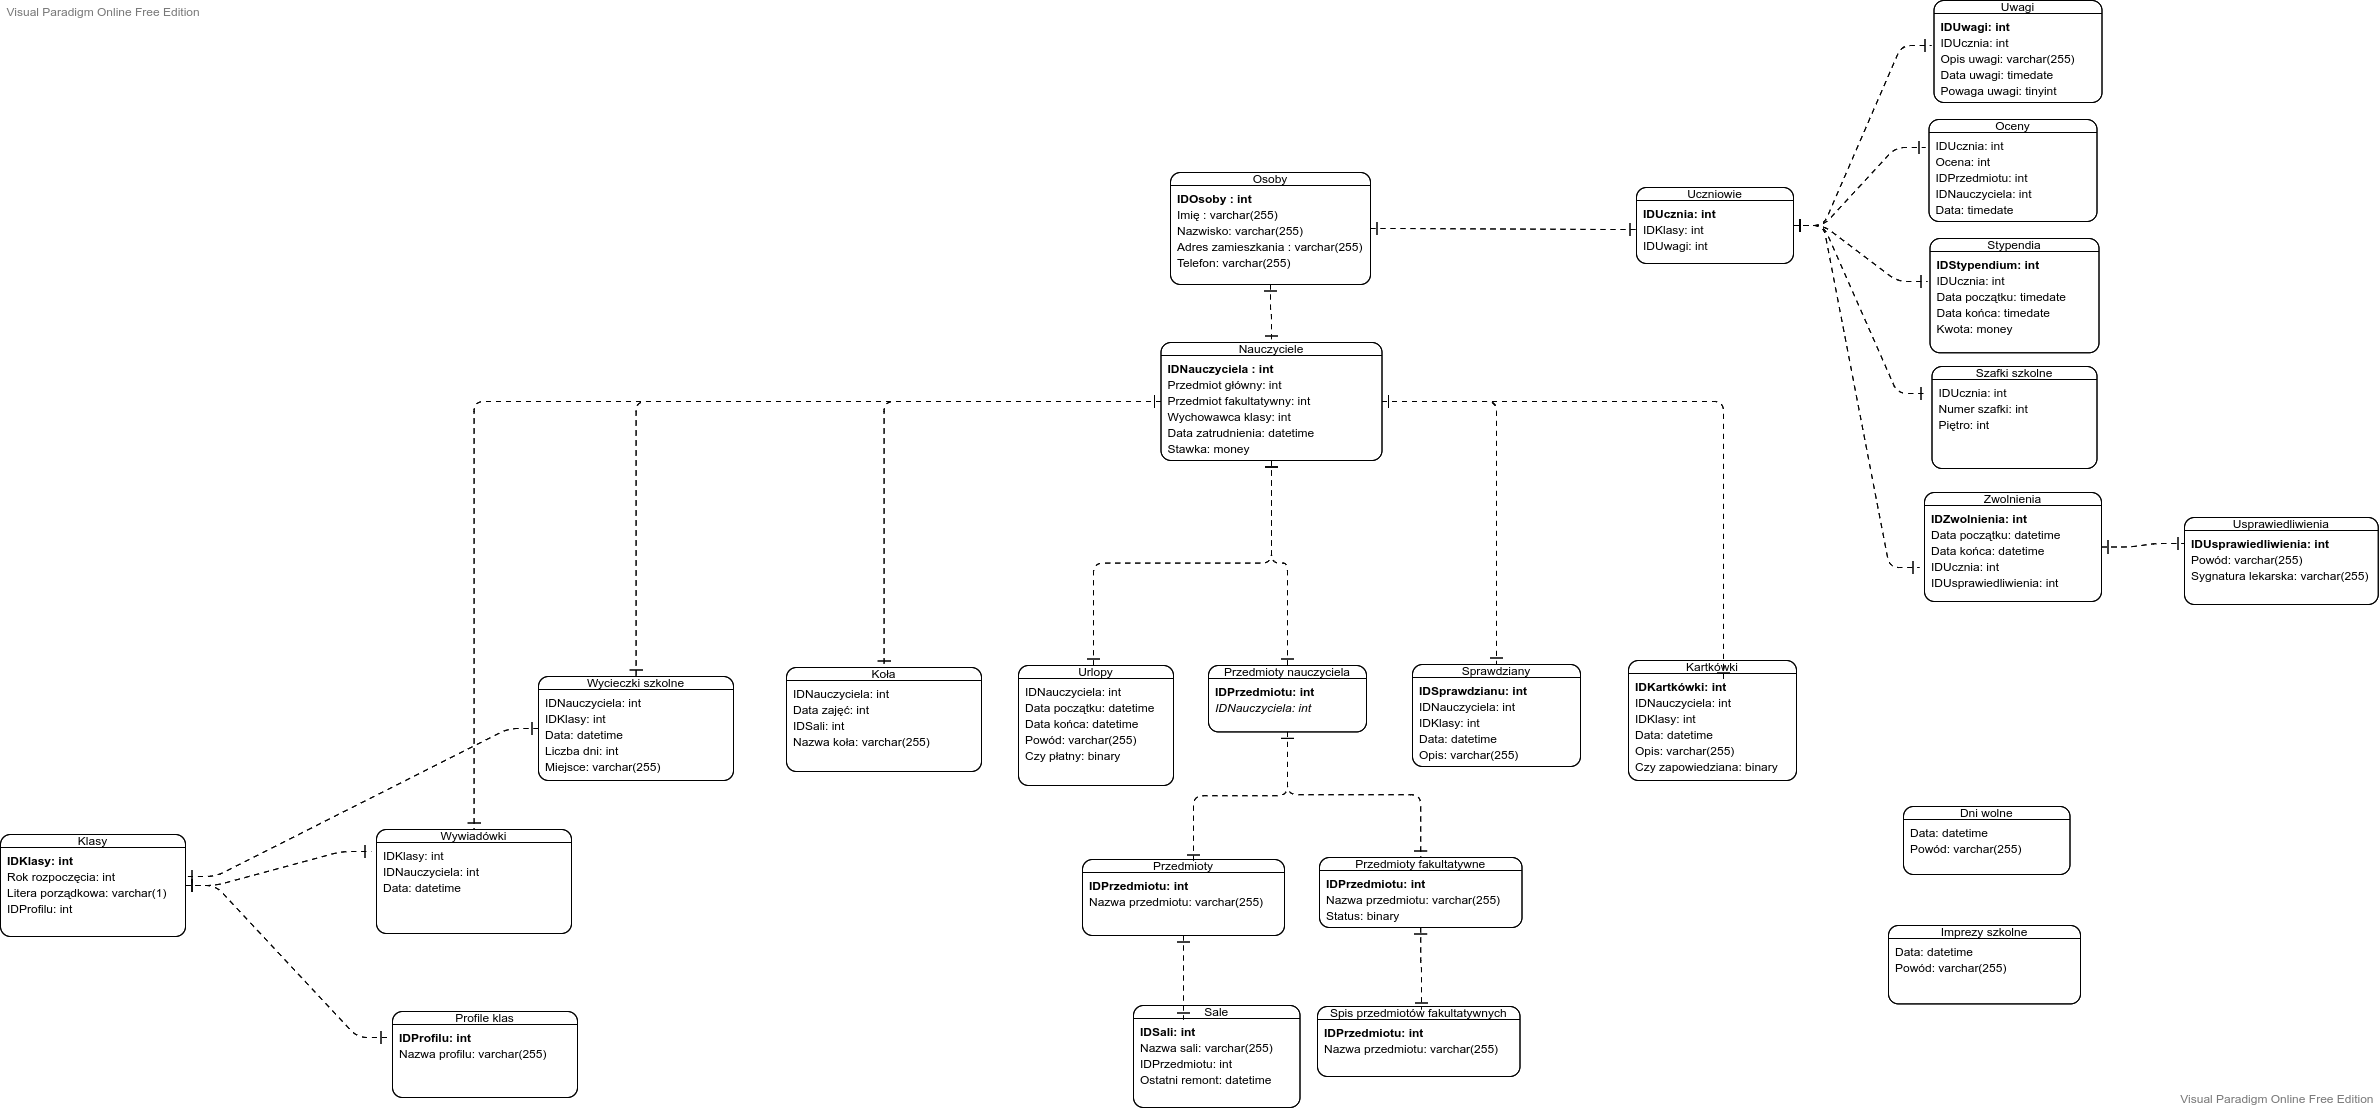
\includegraphics[width=\linewidth]{diagram_ER.png}
  \caption{Diagram ER}
  \label{Diagram ER}
\end{figure}

\subsection{Schemat bazy danych}

\newpage
\section{Dokumentacja technicza}

\subsection{Tabele}

Wymagania: 8 poprawnie zaprojektowanych tabel (na osobę).

\begin{minted}{sql}
    --tworzenie tabeli
    CREATE TABLE Pracownicy
    (
        Nazwa VARCHAR(255) NOT NULL PRIMARY KEY
    );
    --dodawanie rzeczy
    INSERT INTO Pracownicy(Nazwa) VALUES
    ('xd'),
    ('whhhat')
\end{minted}
 
\subsection{Widoki oraz funkcje}

Wymagania: 10 widoków lub funkcji.

\subsection{Procedury i wyzwalacze}

Wymagania: baza danych powinna być odpowiednio oprogramowana z wykorzystaniem procedur składowanych i wyzwalaczy (co najmniej po 5 procedur i po 5 wyzwalaczy).

\end{document}